%%%%%%%%%%%%%%%%%%%%%%%%%%%%%%%%%
%
%       EXERCÍCIO
%
%%%%%%%%%%%%%%%%%%%%%%%%%%%%%%%%%

\ifdefstring{\atividade}{prova}{%
    \ifdefstring{\modo}{objetivo}{%
        \renewcommand{\valorquestao}{\ValorQObj\ ponto}
    }{%
        \renewcommand{\valorquestao}{\ValorQDisc\ pontos}
    }%
}%

\begin{exercicioBanco}[\valorquestao]
Dois objetos metálicos, ambos com temperatura inicial igual a \(10\,^\circ\text{C}\), são aquecidos. Suas temperaturas, \(y_{1}\) e \(y_{2}\), em função do tempo \(t\), em segundo, estão representadas no plano cartesiano pelas semirretas com origem no ponto \(A = (0,10)\) e que passam, respectivamente, pelos pontos \(B = (20, 50)\) e \(C = (40, 30)\). Sabe-se que, em determinado intervalo de tempo, a temperatura \(y_{1}\) aumentou \(20\,^\circ\text{C}\).  

%
\begin{center}
    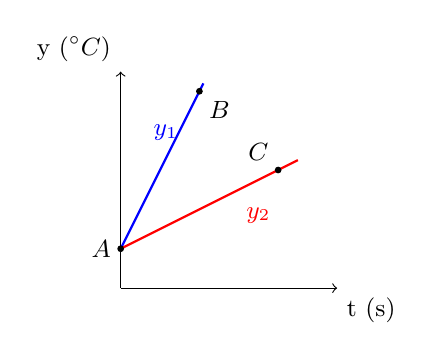
\begin{tikzpicture}[scale=0.5]
        % Eixos
        \draw[->] (0,0) -- (5.5,0) node[below right] {\small{t (s)}};
        \draw[->] (0,0) -- (0,5.5) node[above left] {\small{y (\(^\circ\text{C}\))}};
        
        % Gráfico
        \draw[domain=0:2.1, smooth, variable=\x, blue, thick] plot ({\x}, {2*\x+1}); \node[blue, above left] at (1.7,3.5) {\small\(y_{1}\)};
        \draw[domain=0:4.5, smooth, variable=\x, red, thick] plot ({\x}, {(1/2)*\x+1}); \node[red, below] at (3.5,2.3) {\small\(y_{2}\)};
             
        % Marcando os pontos
        \filldraw (4,3) circle (2pt) node[above left] {\small\(C\)};
        \filldraw (2,5) circle (2pt) node[below right] {\small\(B\)};
        \filldraw (0,1) circle (2pt) node[left] {\small\(A\)};
    \end{tikzpicture}
\end{center}
%

Nesse mesmo intervalo de tempo, determine quanto aumentou a temperatura \(y_{2}\), em grau Celsius.

% Define as alternativas
\newcommand{\alternativas}{%
    \begin{center}
        \begin{tabularx}{\textwidth}{XXXXX}
            (a) \(5\). &
            (b) \(10\). &
            (c) \(15\). &
            (d) \(20\). &
            (e) \(25\).
        \end{tabularx}
    \end{center}
}

% Resposta correta
\newcommand{\resposta}{A}

% Lógica condicional para exibição
\ifdefstring{\atividade}{lista}{%
    \alternativas
    \vspace{0.5em}
    
    \noindent\textbf{Resposta:} letra \textbf{\resposta}.
}{%
    \ifdefstring{\modo}{objetivo}{%
        \alternativas
    }{%
        % modo = discursiva → não mostra alternativas
    }
}
\end{exercicioBanco}

